


\chapter{Översikt över systemet}

\label{Systemet} 

\lhead{Kapitel 2. \emph{Översikt över systemet}}

Systemet ger användaren möjligheten att observera simuleringen av en virtuell myrkoloni i realtid.

Användaren startar simuleringen utan input-parametrar och systemet körs sedan automatiskt och kräver ingen interaktion från användaren. 
Vid första anblick kan myrkolonin uppfattas som simpel, men komplexiteten i simuleringen ligger i systemarkitekturen och de algoritmer myrorna använder sig av för att effektivisera hämtningen av mat. Systemarkitekturen kommer att presenteras mer detaljerat i en annan sektion av rapporten.

\section{Concurrency}

På grund av den höga nivån av autonomitet kombinerat med separationen mellan de olika processerna så är vi tvungna att använda så kallad \emph{event-driven programming}, vilket är när ett program styrs av externa händelser som inte går att kontrollera eller förutse. Ett exempel på det är vid programmering av användargränssnitt, då det inte går att förutspå när eller i vilken ordning användaren kommer att ge input till systemet. 

Vi använder actor-modellen då den ger oss bra möjligheter att på ett konceptuellt och effektivt sätt implementera event-driven programming. Vi kan i actor-modellen fokusera på en modul i taget utan att behöva ta hänsyn till hur de andra modulerna är implementerade. Det enda som behövs är ett meddelandeprotokoll som alla moduler följer.

Det är viktigt att påpeka att vi använder asynkron event-driven programming. Detta ger upphov till många problem då vi inte kan garantera att meddelandena kommer i rätt ordning. Problemen löses med hjälp av meddelandefiltrering, som innebär att en process väntar på ett specifikt meddelande innan den går vidare och buffrar de meddelanden som kvarstår. Varje process behöver då ha ett speciellt tillstånd när den accepterar alla nya förfrågningar.
Simuleringen skapar ofta deadlocks och vi har därför implementerat ett system för att åtgärda dessa. Metoden beskrivs mer detaljerat i kapitel \ref{ch:Implementation}.

\section{Systemdesign}

I figur \ref{fig:design} syns en schematisk överblick av systemarkitekturen. Alla moduler arbetar helt asynkront och all kommunikation mellan modulerna sker via medelanden.

\begin{figure}

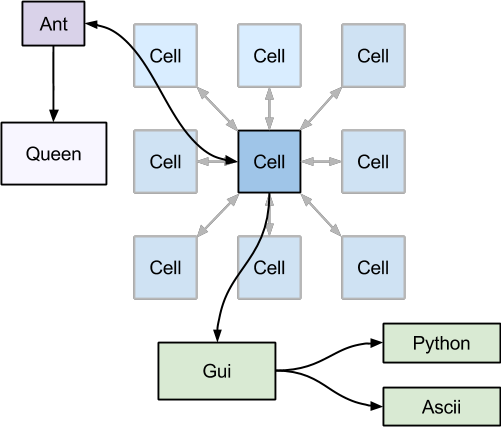
\includegraphics[scale=0.8]{Figures/systemdesign.png}
\caption{En schematisk överblick över systemarkitekturen}
\label{fig:design}
\end{figure}

\subsection{Ant}

Ant-modulen är den modul som implementerar myran. Ant-modulen innehåller de funktioner som krävs för att myran skall kunna fatta beslut över hur den ska agera baserat på hur dess omgivning ser ut. Myran skickar endast förfrågningar till den cell som den befinner sig på. Under normal drift så tar myran aldrig emot några förfrågningar från någon annan process, den tar endast emot svar från den cell som den befinner sig i.

Myran kommer på eget bevåg att skicka förfrågningar till den cellen den står på och autonomt att fatta beslut om vilken handling som är lämpligast, baserat på den informationen myran har tagit del av.

Ant-modulen är utrustad med funktionalitet så att myran kan analysera den information som ges av grannskapet till cellen den står i. Informationen gör det möjligt för myran att fatta ett beslut, baserat på vad myrans omgivning består av. Myror i det verkliga livet kommunicerar med varandra genom olika typer av feromoner, detta för att meddela var maten finns. Det är viktigt att myrorna kan inspektera sin omgivning så att den kan fatta ett beslut baserat på vad andra myror har upptäckt i omgivningen. Finns det feromoner som indikerar till myran att det finns föda i närheten kan myran ta ett beslut att röra sig i den riktningen och leta rätt på födan. Myrorna använder sig även av feromoner för att hitta hem till sitt näste. 


\subsection{Cell}

Cell-modulen representerar cellerna, varje cell är en ruta i det rutnät som utgör världen där myrorna lever. En cells primära uppgift är att ta emot och besvara förfrågningar från myran som står på cellen, samt de kringliggande cellerna. En cell kommer under normal drift aldrig att skicka en begäran till en annan cell, förutsatt att det är inte en begäran för att hantera en förfrågan som cellen har tagit emot. En cell kan endast skicka förfrågningar till de celler som är i dess direkta grannskap.

Cellen är det objekt som innehåller den relevanta informationen för systemet. En cell innehåller information om vad det är för typ av cell, om cellen exempelvis representerar ett myrbo: huruvida det finns mat på cellen, vad för intensitet de olika feromonerna har på cellen och om det står en myra på cellen.

Cellerna är de enda objekten som kommunicerar med GUI-modulen. När en cell får en förfrågan som förändrar cellens tillstånd skickar cellen ett meddelande till GUI-modulen där den talar om sin position och sitt nya tillstånd. 

\subsection{Message\_Buffer}

Message\_Buffer är den modul som hanterar kommunikationen av meddelanden mellan processerna. Modulen exporterar receiver-funktionen, funktionen är central för att använda den typ av event-driven programming som vi arbetar med. Receiver-funktionen används till våra metoder för att hantera deadlocks och filtrering av meddelandekön.

\subsection{GUI}

GUI-modulen är implementerad i Python och Erlang med hjälp av ErlPort. Modulen tar emot och behandlar meddelanden innehållandes cellernas tillstånd från cellerna. 
Informationen omvandlas till Pythons syntax via Erlport och skickas till en Python-instans som hanterar den grafiska representationen.

\subsection{Grid\_Init}

Modulen används för att bygga upp världen samt placera alla celler och länka ihop dessa. Grid\_Init modulen tilldelar även alla celler dess initiala attribut samt skapar, placerar och startar alla myrorna.

I denna modul initieras även en Queen-process, denna process binds alla myror till. Myrorna skickar statistik till Queen-processen, modulen är till för debugging och prestandamätning. 
